\documentclass[thesis.tex]{subfiles}

\begin{document}

\chapter{Design}\label{chap:design}

\section{Erarbeitung aller Funktionen}\label{chap:funktionen}
Nach Auswertung der Anforderungen lassen sich folgende Funktionen herausarbeiten, die der Lone-Worker-Modus leisten soll.
\begin{itemize}
    \item Verbindungsaufbau und Verbindungsabbau sowie Wiederherstellung einer verlorenen Verbindung,
    \item Alarmierung des Alleinarbeiters und des Überwachungszentrums,
    \item Abrufen von Echtzeit Audio- und Videostreams,
    \item Zweiwege-Sprachkanal,
    \item Positionsübermittlung zur Standortüberwachung und für Geofencing,
    \item Übermittlung von Textnachrichten.
\end{itemize}

Die Grundfunktionalität des Lone-Worker-Modus ist die Sicherstellung einer ununterbrochenen Verbindung zwischen dem Alleinarbeiter und einem Überwachungszentrum über die Body-Cam.
Um das sicherzustellen, wird ein zuverlässiger Verbindungsaufbau und -abbau beim Einschalten oder Ausschalten der Body-Cam nötig.
Um nach Aktivierung des Lone-Worker-Modus eine durchgängige Verbindung zu gewährleisten, muss das Programm einen Verbindungsverlust innerhalb weniger Sekunden feststellen.
Danach soll automatisch mit dem Wiederaufbau der Verbindung fortgefahren werden.
Hierzu verbindet sich die Body-Cam nach Einschalten mit einer vorher eingestellten URL, dem Überwachungszentrum.
Beim Anmelden übermittelt sie wichtige Informationen, wie Identifikationsnummer, Standort sowie die Dauer nach dem bei einem Verbindungsverlust der Alarm ausgelöst wird.
Diese Verbindung dient vorerst der Anmeldung und Positionsübermittlung ohne ununterbrochene Verbindungsüberwachung und kann jederzeit vom Alleinarbeiter beendet werden.
Beim Beenden der Verbindung wird diese abgebaut und die Body-Cam meldet sich beim Überwachungszentrum ab.
Wenn ein Verbindungsverlust eintritt, wird eine automatische Wiederherstellung ohne Alarmauslösung ausgeführt.
Bei eingeschaltetem Lone-Worker-Modus geht die Verbindung in einen strengeren Zustand über.
In diesem wird ein Verbindungsverlust unmittelbar festgestellt und geht auf beiden Seiten mit Auslösung eines Alarms einher, falls die Verbindung in einer vorher definierten Zeit nicht wiederhergestellt werden kann.

Die Alarmierung besteht aus einer Alarmmeldung, die auf beiden Seiten der Verbindung dargestellt wird.
Sie kann visuell, akustisch und haptisch sein.
Die Meldung soll dazu dienen den Träger der Body-Cam sowie einen Operator in einem Überwachungszentrum über ein bestimmtes Ereignis zu informieren und die Aufmerksamkeit auf dieses zu lenken.
Diese können von einfachen aber wichtigen Informationen wie Akkustand oder das Verlassen oder Betreten eines bestimmten Bereiches, über kritische Meldungen wie Gefahrensituationen oder eine längere unterbrochene Verbindung gehen.
So kann der Lone-Worker den Alarm beispielsweise durch ein lautes Piepen ähnlich einem Feuermelder, durch Vibration der Body-Cam, durch schnell blinkende LEDs bzw. des Displays oder einer Mischung aus diesen Szenarien erkennen.
Das hat den Vorteil, dass der Träger in jeder Situation optimal informiert werden kann.
Die Vibration des Gerätes kann als stiller Alarm genutzt werden.
So wird der Lone-Worker auf eine bestimmte Situation aufmerksam gemacht, ohne die Aufmerksamkeit der Umgebung auf ihn zu lenken.
Für das Überwachungszentrum spielen diese unterschiedlichen Möglichkeiten keine tragende Rolle.
Hier kommen nur visuelle und akustische Meldungen zum Einsatz, die einen möglichen Operator über eine Situation alarmieren sollen.
Die Priorität der Alarmmeldungen kann durch die unterschiedlichen Möglichkeiten und deren Intensität gesteuert werden.
Z.~B. bekommt der Lone-Worker und das Überwachungszentrum eine kurze Meldung auf dem Display bzw. Monitor begleitet von einem kurzen Piepton, wenn der Akkustand des Geräts unter 25 Prozent fällt.
Dies zählt damit zu den unwichtigeren Meldungen und soll die Beteiligten nur für bevorstehende Ereignisse sensibilisieren.
Die Intensität dieser Meldung steigt, wenn der Akkustand einen kritischen Punkt erreicht.
Hierzu könnten dann lautere und längere Pieptöne sowie eine Vibration der Body-Cam genutzt werden.
Wenn ein akuter Gefahrenfall auftritt, sollte sich die Alarmmeldung signifikant von anderen unterscheiden, um damit die volle Aufmerksamkeit des Lone-Workers und des Überwachungszentrums auf die Situation zu lenken.

Der Abruf von Echtzeit-Audio- und Videostreams soll ebenfalls von der Body-Cam umgesetzt werden.
Eine Video- und Audioaufzeichnung sowie die Möglichkeit, diese zu streamen bietet die Body-Cam bereits, wie in \autoref{chap:grundlagen} beschrieben.
Diese Option soll auch für den Lone-Worker-Modus zur Verfügung stehen.
Dabei kann ein Operator eine Anfrage an eine Body-Cam stellen, um die jeweiligen Streams vom Gerät abzurufen und im Überwachungszentrum anzeigen zu lassen.
Diese Möglichkeit kann vor allem im Bereich einer Mobilfunkverbindung nur eingeschränkt nutzbar sein.
So müssen hier aufgrund von Verbindungsstärke und -qualität Einbußen bei Verfügbarkeit und Qualität der Streams gemacht werden.
Bei einer guten WLAN-Abdeckung, wie sie in Gebäuden eingesetzt werden kann, besteht dieses Problem weniger.
Hier kann durch die Nutzung einer WLAN-Verbindung eine wesentliche höhere Bandbreite und Verbindungsstärke genutzt werden.
% Außerdem haben Unternehmen die Möglichkeit die Abdeckung ihrer WLAN-Verbindung auszubauen, um eine bessere Qualität der Verbindung zu gewährleisten.
% Diese Option besteht bei der Nutzung der öffentlichen Mobilfunknetze nicht.

Neben einer aktiven Anfrage durch das Überwachungszentrum kann der Stream bei Bedarf auch im Alarmfall übertragen werden.
Hierfür kann die Body-Cam automatisch die Streams an das Zentrum übertragen, wenn der Lone-Worker einen Alarm auslöst.
Dies hat den Vorteil, dass der Operator nach Eingang einer Alarmmeldung sofort die Möglichkeit hat, sich ein Bild von dem Gefahrenfall zu machen.
Er kann dafür die Informationen aus Bild und Ton nutzen, um die Situation besser einzuschätzen und bei Bedarf weitere Schritte einzuleiten.

Um den Informationsaustausch weiter zu verbessern, baut die Body-Cam nach Bedarf einen Zweiwege-Sprachkanal zwischen dem Operator und dem Lone-Worker auf.
Dieser ermöglicht einen aktiven Austausch zwischen Träger und Empfangseinrichtung.
Der Austausch von Informationen findet damit nicht mehr nur einseitig in Richtung des Überwachungszentrums statt.
So hat der Lone-Worker die Möglichkeit, sich mit einem Operator über verschiedene Sachverhalte auszutauschen und Klarheit über eine Situation zu schaffen.
Unter anderem kann das zur Minderung des Isolationsgefühls beitragen \cite[vgl. S.~45][]{GeyerMagiera2022}.

Eine weitere Funktion ist die Standortübermittlung.
Die Body-Cam übermittelt kontinuierlich ihren Standort an das Überwachungszentrum.
Die Genauigkeit der Position wird durch die Verbindung von GPS, Mobilfunk, WLAN und Bluetooth erhöht.
Dies ist in erster Linie wichtig um bei einem Notfall den exakten Standort der in Gefahr befindlichen Person zu detektieren.
So können Notfallkräfte im Ernstfall schnell und gezielt reagieren.
Ein weiterer Vorteil dieser Positionsüberwachung ist das sogenannte Geofencing.
Dies beschreibt das automatische Auslösen bestimmter Aktionen beim Ein- oder Austritt aus einem vorher festgelegten Bereich \cite[]{geofencing}.
Damit wäre es möglich Bereiche für Schichtbeginn und -ende oder mit besonders hohen Gefahrenpotenzial zu markieren.
Der Lone-Worker würde dann bei Betreten über diesen Umstand per Body-Cam informiert werden, damit er die volle Konzentration auf seine Sicherheit lenken kann.
Zusätzlich kann die Standortüberwachung in die Protokollierung der Alleinarbeit mit einfließen, um diese mit Informationen über Laufwege und Aufenthaltsdauer zu verbessern.

\begin{figure}[h]
    \centering
    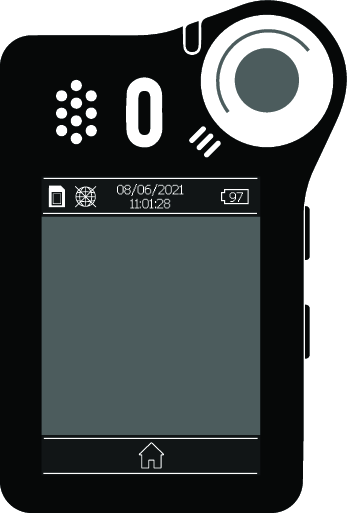
\includegraphics[height=0.4\textwidth]{/BC_schema_front.png}
    \caption[Schemata der Front einer Body-Cam]{Schemata der Front einer Body-Cam \cite{netco}}
    \label{fig:BC_schema}
\end{figure}

Durch das vorhandene gezeigte Display mit Touch-Funktion besteht die Möglichkeit zum Anzeigen und Beantworten von Textnachrichten.
Mit den Nachrichten kann das Überwachungszentrum dem Lone-Worker kurze Informationen übermitteln oder nach dem Status fragen, ohne eine Sprachverbindung zu benutzen.
Die Beantwortung kann der Träger über vorher definierte Antworten übernehmen, die als Buttons auf dem Display erscheinen.
Automatisch generierte Textnachrichten können zur Unterstützung genutzt werden.
Sie können nach bestimmten Ereignissen mehr Informationen bereitstellen.
Zu diesen Events zählen beispielsweise Alarmauslösung, Ein- oder Austritt aus einem Geofencing-Bereich, Fehlfunktionen oder Statusveränderungen der Body-Cam.
Außerdem wird das in \autoref{fig:BC_schema} gezeigte Display dafür genutzt, alle möglichen Statusinformationen über das Gerät anzuzeigen, wie Akkustand, Mobilfunkstärke oder Temperatur.

\section{Protokolldesign}\label{chap:protokolldesign}
Damit alle Anforderungen an die Kommunikation zwischen Body-Cam und Überwachungszentrum erfüllt werden können, wird ein eigenes Protokoll verwendet.
Dieses wird in der einheitlichen und weit verbreiteten „JavaScript Object Notation“ (JSON) verfasst.
Dieser Standard hat für die Anwendung folgende Vorteile.
Das Protokoll kann einfach zwischen Client und Server übertragen werden, da JSON sehr einfach in einen String umgewandelt werden kann.
Es existieren bereits in vielen Programmiersprachen Bibliotheken die JSON verstehen, bearbeiten und umwandeln können, welche Nachrichten schnell zwischen verschiedenen Anwendungen konvertieren können, wenn dies benötigt wird.
Das Protokoll kann durch diese Form einfach und schnell erweitert oder angepasst werden.
Durch seine einheitliche Struktur und Hierarchieebenen wird dieser Effekt verstärkt und die Nachrichten können dadurch gut strukturiert werden.
Es ist menschenlesbar und kann somit ohne spezielles Programm von Menschen gelesen und verstanden werden.
Dies hilft z.~B. beim Debuggen oder um Protokolleinträge schneller lesen zu können. \cite[]{ecma_404}

Das entwickelte Protokoll enthält folgende Informationen: Zeitstempel, Referenznummer, Nachrichtentyp, Nachrichteninhalt, Antwortreferenznummer.
Der Zeitstempel wird der Nachricht beim Erstellen gegeben, damit der zeitliche Verlauf nachvollzogen werden kann und die Nachrichten in einem Verlaufsprotokoll angelegt werden können.
Die Referenznummer wird aufsteigend für jede Nachricht vergeben und macht diese eindeutig identifizierbar.
Diese Nummer wird auch als Referenznummer für eine Antwort auf eine bestimmte Nachricht genutzt.
Diese wird dann unter Antwortreferenznummer der Nachricht mitgeben und findet nur bei Nachrichten des Typs Answer Anwendung.
Der Nachrichtentyp gibt an, welchen Typ die geschickte Mitteilung hat.
Hier gibt es momentan die Typen Request, Answer, Heartbeat und initialMessage.
Heartbeat wird immer dann vergeben, wenn ein Nachrichtenaustausch zwischen Client und Server stattfindet, der zur Verbindungssicherung dient.
Die initiale Nachricht schickt der Client einmalig am Anfang einer Verbindung an den Server, um ihm Einstellungs- und Verbindungsparameter mitzuteilen.
Im Nachrichteninhalt befindet sich alles, was die Mitteilung als Daten beinhaltet.
Dies können beispielsweise gerade genannte Parameter oder Anfrage- bzw. Antwortdetails sein.
Durch den Aufbau der JSON kann das Datenfeld bei Bedarf ebenfalls strukturiert werden, um auch größere Datenmengen gut abbilden zu können.

\section{Primitiven}\label{chap:primitiven}
% https://www.itwissen.info/Primitive-primitive.html
Im folgenden Kapitel werden alle Primitiven aufgeführt und beschrieben.
Als Primitiven sind alle Informationen zu verstehen, die zwischen Lone-Worker-Modus und der bestehenden Body-Cam ausgetauscht werden, um die vollständige Funktionsfähigkeit zu gewährleisten.
Sie sind die Schnittstellen, über die der Modus beispielsweise Geräteinformationen abrufen kann.

Um die Grundfunktionalität des Geräts und den damit verbundenen Lone-Worker-Modus sicherzustellen, werden in erster Linie
die Vitalwerte des Geräts sowie Verbindungsinformationen benötigt.
Es müssen jedoch alle Informationen bereitgestellt werden, die für den Einsatz als Alleinarbeitslösung notwendig sind.
Darunter zählen unter anderem:
\begin{itemize}
    \item eindeutige Identifikationsnummer der Body-Cam,
    \item aktuelle Versionsnummer der Firmware und Software,
    \item aktueller Zeitstempel,
    \item Batteriezustand,
    \item vorhandene Speicherplatz für Bild- und Videodateien,
    \item Temperatur,
    \item Mobilfunkstärke sowie Informationen über die Mobilfunkverbindung,
    \item WLAN-Stärke und dazugehörige Verbindungsdetails,
    \item Bluetooth- und WLAN-Geräte in der Nähe,
    \item letzte bekannte Standorte.
\end{itemize}

Informationen, die sich schnell ändern können, wie Verbindungsdetails und -stärken, der letzte Standort und
einen aktuellen Zeitstempel sollen alle 1-5 Sekunden, von der Body-Cam abgefragt werden können.
Batteriestatus, Temperatur und Speicherplatz die zum Überwachen des Gerätezustands wichtig sind, sollten alle 30 Sekunden zur Verfügung stehen.
Einmalig zum Start der Software werden Versions- und Identifikationsnummern benötigt, da diese Angaben sich während des Betriebs nicht ändern können.

Der Lone-Worker-Modus muss im Alarmfall die Lautsprecher, den Vibrationsmechanismus sowie die LEDs ansteuern können.
Dies wird benötigt, um die akustischen, haptischen und visuellen Alarmmeldungen an den Lone-Worker weiterzureichen.
Der Lautsprecher wird neben dem Abspielen von Alarmtönen noch für das Abspielen von Audionachrichten verwendet.
Das Display wird wie in \autoref{fig:BC_schema} gezeigt für das Anzeigen von Statusinformationen genutzt.
Auf dem freien Platz in der Mitte soll der Lone-Worker-Modus die Möglichkeit haben, eigene Informationen anzuzeigen.
Das sind z.~B., der aktuelle Zustand des Modus, Textnachrichten des Überwachungszentrums oder Alarmursachen.

Der Lone-Worker-Modus muss die Möglichkeit haben, Kamera und Mikrofon in Verbindung mit dem Video- und Audiostream zu aktivieren.
Auf Anfrage des Überwachungszentrums soll die Body-Cam die beiden Streams über eine gesicherte Verbindung zur Verfügung stellen.
Außerdem soll dies nach gleichem Schema auch für die Zweiwege-Audio-Verbindung vollzogen werden.
Diese realisiert eine aktive Sprachverbindung zwischen Operator und Lone-Worker.

% \pagebreak

\section{Statemachine}

\begin{figure}[h]
    \centering
    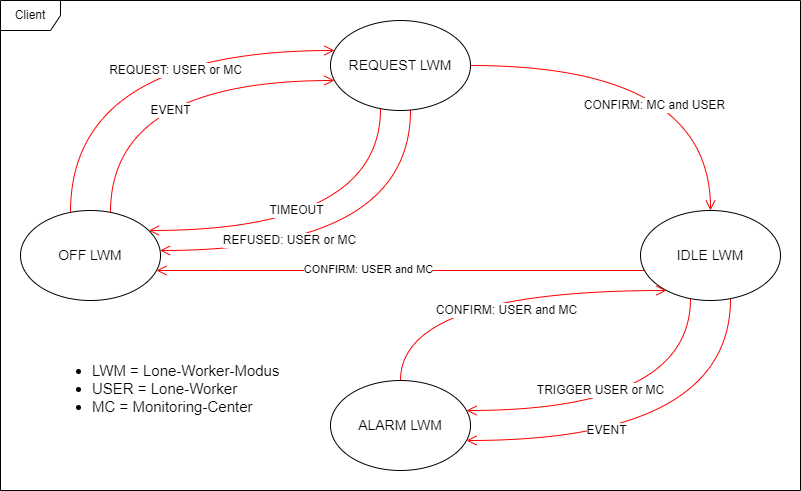
\includegraphics[width=1\textwidth]{/Statemaschine_Client.png}
    \caption[Statemaschine der Client-Seite]{Statemaschine der Client-Seite \lbrack eigene Darstellung\rbrack}
    \label{fig:statemachine}
\end{figure}

Zur Vorbereitung auf die Implementierung des Lone-Worker-Modus wurde eine einfache Statemachine für die Client-Seite angefertigt.
\autoref{fig:statemachine} zeigt die vier Zustände, die der Modus annehmen kann und in welchen Fällen sich dieser ändert.
Der Wechsel zwischen dem inaktiven und aktiven Lone-Worker-Modus wird durch einen Request-Zustand unterbrochen.
Dieser kann durch eine manuelle Anfrage von dem Träger der Body-Cam oder dem Überwachungszentrum sowie durch ein Event betreten werden.
Ein Event ist in diesem Zusammenhang beispielsweise die automatische Aktivierung durch das Betreten eines Geofencing-Bereiches.
Nach einer Anfrage zur Aktivierung muss diese durch beide Seiten bestätigt werden.
Bei einer manuellen Auslösung einer Partei gibt diese automatisch das Einverständnis zum Einschalten des Modus.

Im Idle-Zustand befindet sich die Body-Cam solange es zu keinem Alarm kommt oder die Verbindung ohne Fehler beendet wird.
Die Verbindung kann durch Bestätigung beider Seiten beendet werden und der Client geht damit wieder in den Off-Zustand über.
Der Alarm-Zustand kann ähnlich zum Request-Zustand wieder durch einen manuellen Auslöser oder durch ein Event betreten werden.
Die Betätigung des roten Alarm-Knopfs der Body-Cam oder eine Alarmmeldung eines Operators im Überwachungszentrum zählt unter die manuelle Auslösung.
In diesem Kontext sind Events z.~B.:
\begin{itemize}
    \item Verbindungsverlust,
    \item Auslösen des Lagesensors,
    \item Betreten oder Verlassen eines Geofencing-Bereiches,
    \item Kritischer Batteriezustand.
\end{itemize}

Zusätzlich zu der Statemachine wurde jeweils ein Zustandsdiagramm für beide Seiten angefertigt.
\autoref{fig:zustandsdiagramm_client} zeigt das Diagramm der Client-Seite.
In diesem wird gezeigt, wie nach einer erfolgreichen Verbindung eine Schleife die Kommunikation zum Server verwaltet.
Das Diagramm stellt den Programmablauf dar, um Anfragen vom Server zu beantworten oder eigene Anfragen, die von der Body-Cam gestellt werden, an den Server zu senden.
Es wird dargestellt wie Anfragen mit Timeouts in eine Warteliste gepackt werden und wie nach jeder Iteration diese Liste auf ausgelaufene Anfragen überprüft wird.
Das soll sicherstellen, dass die über die Schnittstellen gestellten Anfragen von der Body-Cam an den Lone-Worker-Modus in endlicher Zeit beantwortet werden können.
Im \autoref{anhang:zustandsdiagram_server} befindet sich das Zustandsdiagramm für die Server-Seite.
Es unterscheidet sich nur geringfügig von dem des Clients und wird deshalb hier nicht weiter vertieft.

\begin{figure}[h]
    \centering
    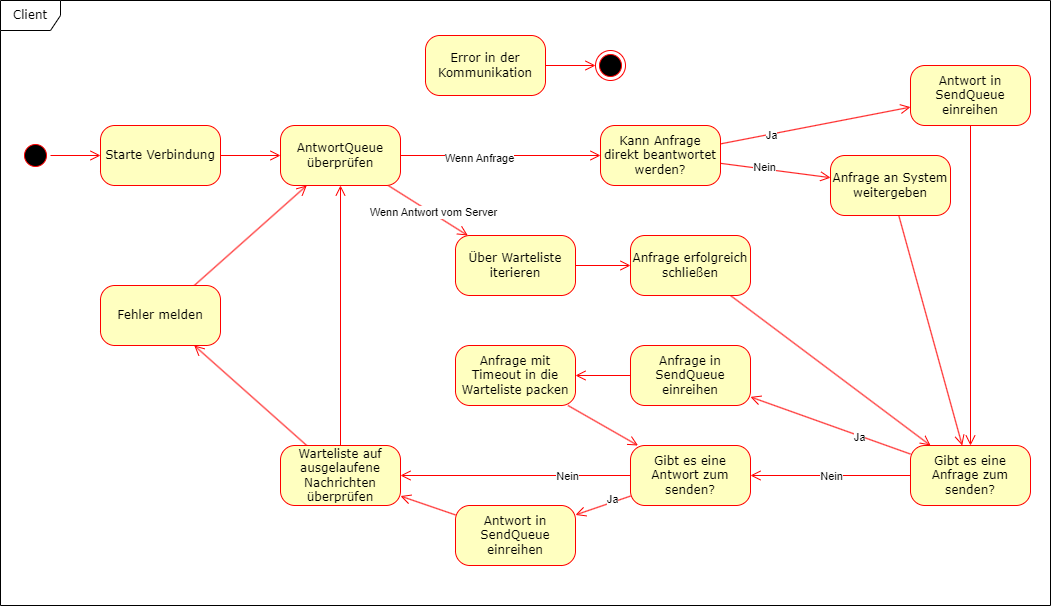
\includegraphics[width=1\textwidth]{/Zustandsdiagramm_Client.png}
    \caption[Zustandsdiagramm der Client-Seite]{Zustandsdiagramm der Client-Seite \lbrack eigene Darstellung\rbrack}
    \label{fig:zustandsdiagramm_client}
\end{figure}

\subfilebib % Makes bibliography available when compiling as subfile
\end{document}